\section{Use of damping materials to de-Q resonant caviities}
\label{sec:damping_materials}

For a number of devices it is unavoidable to have a cavity present in the structure. In addition it is often not possible to design the cavity with either tapering or transition pieces due to the need for moveable components, such as a wire scanner or a collimator whose aperture changes with beam parameters. In this case it is necessary to find a way of reducing the beam impedance by altering the properties of resonances. Often it is only the peak value of the impedance attributable to a resonance that is of concern from a beam stability/beam induced heating point of view. 

If we consider the defining properties of a resonant impedance, $f_{res}$, $R/Q$ and $Q$, there are a number of properties that should be noted in changing them. Both $f_{res}$ and $R/Q$ are strongly determined by the geometry of the structure, and thus can not be significantly modified without possibly neccessitating a modification of the device being altered which may hinder the intended operation. Thus one approach to use is to alter the Q of the resonance. A well known method of altering the Q of a resonant cavity is to add a dispersive or ferritic material to the cavity volume \cite{Klingbeil:ferrCav}, that is a material that has complex permitivitty or permeability , given by $\epsilon_{r} = \epsilon^{'} - j \epsilon^{''}$ and $\mu_{r} = \mu^{'} - j \mu^{''}$ respectively. An example of the permeability of some sample ferrite damping materials is shown in Fig.~\ref{fig:ferr_mu_damp}

\begin{figure}
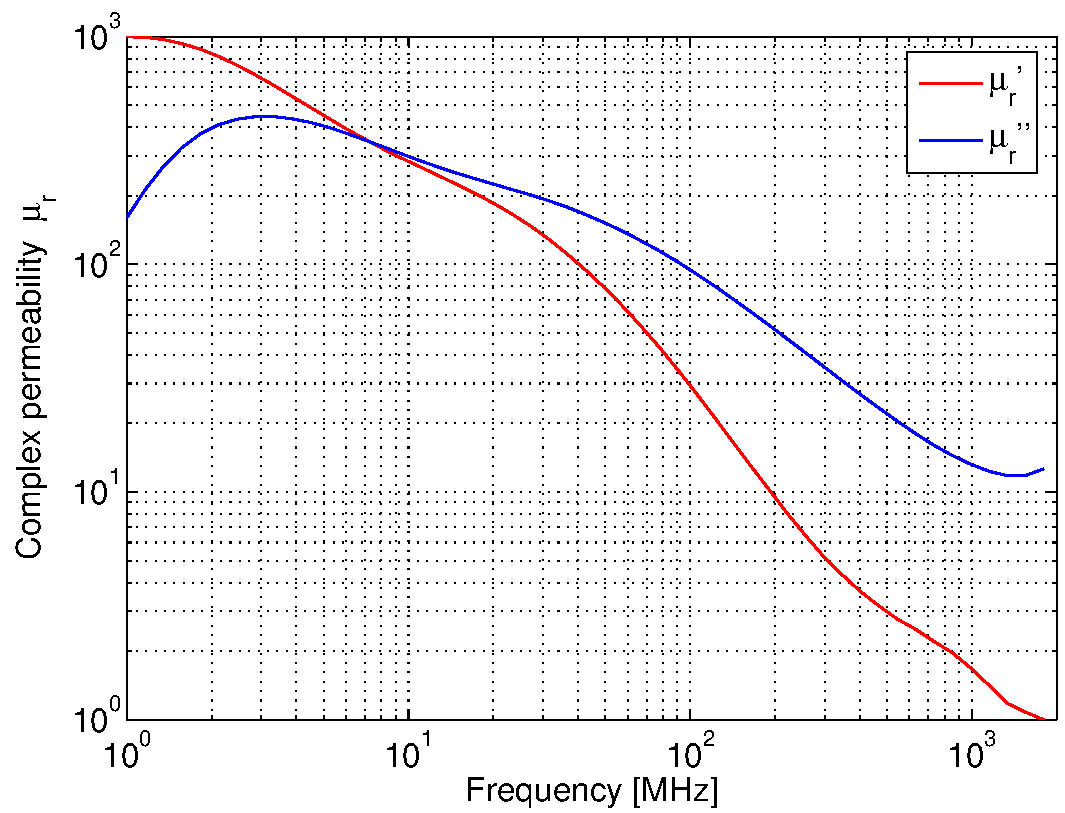
\includegraphics[width=0.6\textwidth]{Beam_Coupling_Impedance_Reduction_Techniques/figures/Ferrite8C11.pdf}
\label{fig:ferr_mu_damp}
\caption{The complex permeability of a sample ferrite of the sort used for damping. In this case 8C11. In use a high $T_{c}$ ferrite is recommended, such as TT2-111R.}
\end{figure}

The addition of this family of materials to the cavity has the following effect on the cavity resonances:

\begin{enumerate}
\item{The resonant frequency of any resonance $\omega_{res}$ is reduced by the inclusion of the dispersive material. This can be understood either by considering the $\mu_{r} / \epsilon_{r}$ increasing the effective electrical volume of the cavity by it's inclusion, thereby increasing the dimensions of the resonant cavity. Alternatively, considering the RLC equivalent circuit of a cavity resonance, the inclusion of the dispersive material increases either or both of (depending the properties of the material) the inductance and capacitance of the cavity.}
\item{The $R/Q$ of the cavity experiences little change. There is a slight modification; either an increase that can be attributed to the increased stored energy in the cavity mode due to $\epsilon^{'} \> 1$ or a decrease due to the reaaranging field patterns (caused by the incluson of the dispersive material) decreasing the stored energy.}
\item{The $Q$ of the resonance is drastically reduced. This is due to the strong change in the damping time of the resonance that the addition of the damping material. In terms of cavity properties this can be thought of as the losses in the cavity increasing more rapidly than the stored energy in the cavity. In equivalent circuit terms this may be thought of as the capacitance of the cavity decreasing or the inductance increasing depending on whether a dielectric or ferrous material is added.}
\end{enumerate} 

As can be seen, the resulting effect is to drastically reduce the $Q$ of a cavity resonance, and then by the relation $R_{s} = R_{s}/Q Q$ it can be seen that the shunt impedance will decrease proportional to $Q$. This reduces the peak of $R_{s}$, but broadens the width of the resonance peak. This indicates two effects of using damping materials as an impedance reduction technique; effects dependent on the shunt impedance $R_{s}$ are suppressed, however effects dependent on the broadband behaviour may suffer negatively as a result. Due to the strong frequency dependent nature of many impedance-driven instability mechanisms and beam-induced heating, these negative side effects rarely outway the benefits using damping material in a cavity if necessary.

\subsection{Heat Loads on the Damping Material}

During experience of estimating the heat loads on ferrite damped cavities in high intensity hadron machines (see Sec.~\ref{sec:tctp} for more details), a number of surprising observations were made. In particular was that the placement of ferrite in a cavity does not always produce a significant reduction in the $Q$ of a resonance and that is such cases the percentage of the power loss in the ferrite was comparatively small compared to conventional wisdom, this being that the ferrite experienced the majority of the heat load of the damped cavity. It was thus decided to investigate how the addition of a damping material, in this case a ferrous material, to a cavity would alter both the characteristic resonance properties of the cavity and the location of the power load due to interaction with the beam in the cavity.

Two different geometries were used, one of which could be treated analytically to provide a benchmark for the simulation code, and one in which the ferrite is shielded from being directly seen by the traversing beam, as is normally done to reduce the effects of a resistive wall type impedance due to the ferrite. These geometries are shown in Fig.~\ref{fig:ferr_cav_res}. A single eigenmode of each cavity is investigated, both with and without a damping material. 

\begin{figure}
\subfigure[]{
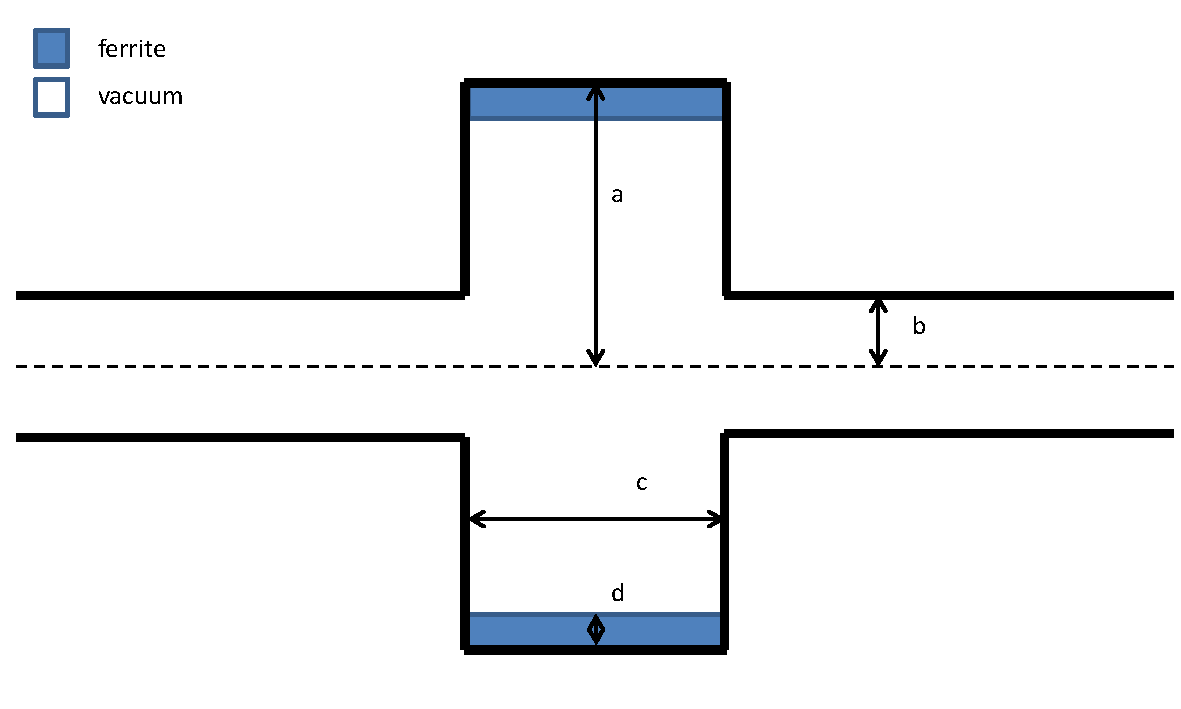
\includegraphics[width=0.45\textwidth]{Beam_Coupling_Impedance_Reduction_Techniques/figures/pillbox_cavity_ferr.pdf}
\label{fig:cav_ferr_no_shield}
}
\subfigure[]{
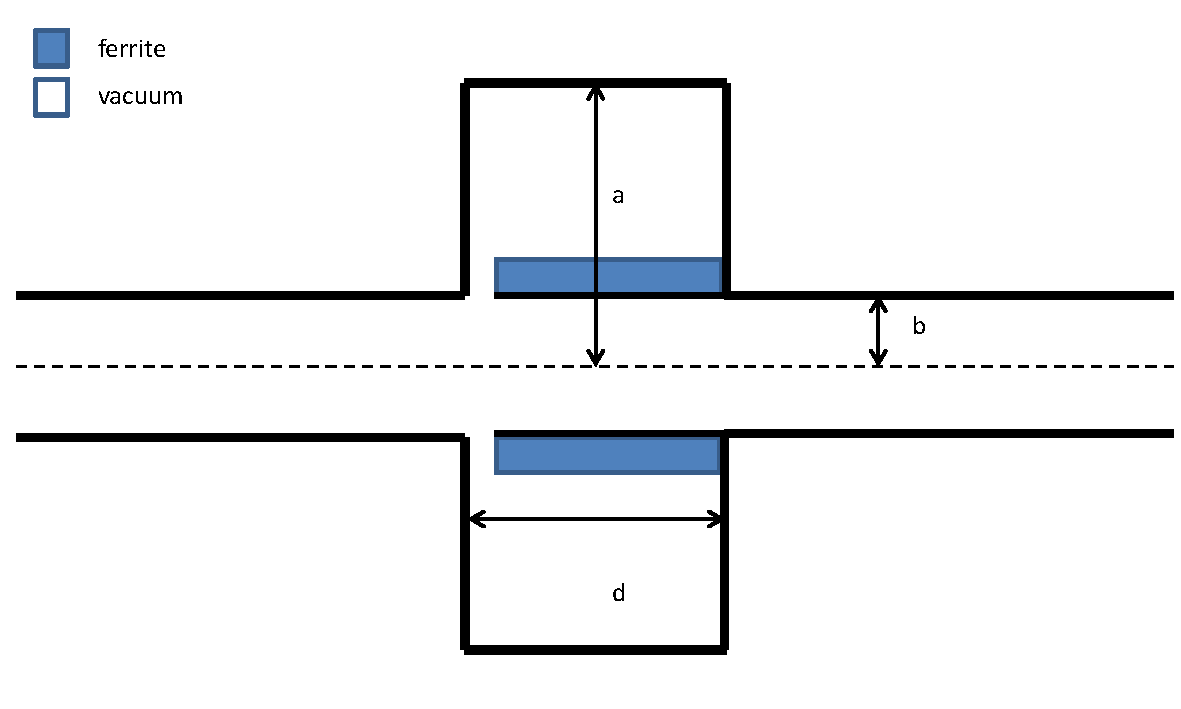
\includegraphics[width=0.45\textwidth]{Beam_Coupling_Impedance_Reduction_Techniques/figures/pillbox_cavity_shielded_ferr.pdf}
\label{fig:cav_ferr_shield}
}
\label{fig:ferr_cav_res}
\caption{Two sample geometries used to examine the effects of ferrite damping material on cavity resonances. \ref{fig:cav_ferr_no_shield} shows a cavity with the ferrite unshielded, and \ref{fig:cav_ferr_shield} shows a more realistic case in which the ferrite is shielded from directly seeing the traversing beam.}
\end{figure}

For this analysis, a cavity of dimensions $a=60mm$, $b=5mm$, $c=20mm$, made from a material with a conductivity $\sigma = 1.1 \times 10^{6} S m^{-1}$ is used for the simulations of an unshielded cavity. A layer of "ferrite" 0.5mm thick is placed as shown in Fig~\ref{fig:cav_ferr_no_shield}. This material is given the following properties: $\epsilon^{'} = 10$, $\epsilon^{''}/\epsilon^{'} = 0$, $\mu^{'}=/1$. $\mu^{''}/ \mu^{'}$ is changed between 0 and 0.02 in steps of 0.02 in order to alter the Q of the resonant mode in incremental steps with the intent of observing how the properties of the cavity change with different scales of damping of the resonance. The "ferrite" is also given a mild conductivity ($\sigma_{ferr} = 10^{-6} S m^{-1}$) as is normal in accelerator ferrites to reduce electrostatic charge build up. 

For the shielded geometry, we use a cavity of the same dimensions as for the unshielded case, with a layer of conductive material 1mm thick placed on the interior of the cavity. A gap of 5mm is left between the beam pipe and the cavity for the beam to couple to the cavity. A ring of ferrite 0.5mm in thickness is then placed on this surface as is shown in Fig.~\ref{fig:cav_ferr_shield}.

Before carrying out the analysis of the location of the heat loss in ferrite, it is prudent verify that the losses calculated using the field calculator in HFSS are self-consistent and well understood. HFSS calculates two losses internally; the surface loss density and volume loss density. The surface loss density $p_{s}$ is defined in HFSS as

\begin{equation}
p_{s} = \Re{}e \left( \mathbf{S}.\mathbf{n} \right)
\end{equation}

where $\mathbf{S}$ is the Poynting vector and $n$ is the out normal vector to the surface boundary \cite{hfss}. By integrating this over all surfaces the total surface losses in the cavity are obtained. The total wall losses are also given by 

\begin{equation}
P_{loss, wall} = \frac{R_{wall}}{2} \int_{S} \left| \mathbf{H_{surf}} \right|^{2} dS
\label{eqn:wall_losses}
\end{equation}

where $R_{wall}$ is the surface resistance of the wall and $\mathbf{H_{surf}}$ is the surface magnetic field.

HFSS defines the volume loss density $p_{v}$ as 

\begin{equation}
p_{v}=\frac{1}{2}\Re{}e\left( \mathbf{E}.\mathbf{J} + \left( -\mathbf{\nabla} \times \mathbf{E} \right).\mathbf{H} \right) 
\label{eqn:vol_loss_density}
\end{equation}

where again this may be intergrated over all space to obtain the total volume losses. In addition to these methods of loss calculations of the losses due to the fields in the cavity, it is possible to calculate an equivalent loss of a particle traversing on axis. By considerations of ohmic losses, with the voltage $V$ that experienced by the particle traversing the cavity, the voltage $R = R_{s}$ the shunt impedance of the cavity resonance and $I$ the beam current. As the eigenmode simulation does not directly simulate a beam, the effective power loss is given by 

\begin{equation}
P_{loss} = \frac{V^{2}}{R_{s}}.
\end{equation}

The surface losses and volume losses are subsequently seperately compared. For the surface losses, the internal surface loss density integrated over all surfaces calculated by HFSS, wall losses as given by Eqn.~\ref{fig:wall_losses} and the equivalent losses of a particle on axis are compared. For this we use the unscreened cavity with no ferrite present to have only surface losses present. The different calculated results are shown in Tab.~\ref{tab:surface_losses_ferr}, given in watts normalised to a peak electric field of $1v m^{-1}$ in the cavity. It can be seen that the two calculations due to the surface fields themselves agree exceptionally well, and the calculation for the equivalent loss of an on-axis particle is agrees to within 20\%. 

\begin{table}
\caption{Comparison of the power loss on the surface of a pillbox cavity by both direct calculation and internal calculation by HFSS (In units normalised to 1V/m maximum electric field)}
\begin{center}
\begin{tabular}{c | c }
Calculation Type & Normalised Power Loss (W)\\ \hline
Direct Calculation & 6.2e-10\\ \hline
HFSS Internal Loss Calculations & 6.22e-10 \\ \hline
Loss of an on-axis particle	 & 5.1e-10 \\
\end{tabular}
\end{center}
\label{tab:surface_losses_ferr}
\end{table}

For the volume losses the cavity geometry for the unshielded case is used, with a layer of ferrite 0.5mm thick on inside surface of the cavity. This ferrite has the following material properties; $\epsilon^{'} = 10$, $\epsilon^{'}=0$, $\mu^{'}=10$, $\mu^{"} / \mu^{"} = 0.1$. For this comparison the internal volume loss density integrated over the whole volume as calculated by HFSS, calculating the volume losses using Eqn.~\ref{eqn:vol_loss_density} and the equivalent loss of an on axis particle are calculated, again with loss normalised to a peak electric field of $1 V m^{-1}$ in the cavity. The results are shown in Tab.~\ref{tab:volume_losses_ferr}. It can be seen that the agreement between all three methods of calculating the losses in the cavity is exceptionally good, differing by less than 10\%.

\begin{table}
\caption{Comparison of the power loss in the volume of a pillbox cavity by both direct calculation and internal calculation by HFSS (In units normalised to 1V/m maximum electric field)}
\begin{center}
\begin{tabular}{c | c }
Calculation Type & Normalised Power Loss (W)\\ \hline
Direct Calculation & 1.28e-8\\ \hline
HFSS Internal Loss Calculations & 1.29e-8 \\ \hline
Loss of an on-axis particle & 1.33e-8 \\
\end{tabular}
\end{center}
\label{tab:volume_losses_ferr}
\end{table}


The resulting real component of the longitudinal beam coupling impedance for the case of unshielded ferrite is shown in Fig.~\ref{fig:no_screen_long_imp}. The change in the resonant frequency and the increase in the peak impedancefrom the cavity without any damping material to that with is due to the presence of a region of $\epsilon_{r}>1$. Clearly seen can be the effect of the presence of increasing loss tangent of the ferrite, greatly broadening the impedance peak, with the effect of reducing $R_{s}$ of the resonance. The cause of this reduction of $R_{s}$ can be attributed to the reduction in $Q$ for each resonance, as shown in Fig.~\ref{fig:cav_ferr_no_shield_tan_v_q}. It can be clearly seen that the presence of a small piece of ferrite very strongly decreases the Q of a resonance. The corresponding change in the percentage of the power loss in the ferrite itself as the Q is decreased is shown in Fig.~\ref{fig:cav_ferr_no_shield_q_v_loss_ferr}. It can be seen that the power loss is rapidly localised to the ferrite as the Q decreases. To quantification to this power loss, the power loss due to this cavity resonance is calculated assuming a beam with $1.15 \times 10^{11}$ particles per bunch, 288 bunches, a ring circumference 6911m and a bunch length $4\sigma = 0.04m$ assuming a gaussian bunch distribution and that the resonance falls on a beam harmonic, shown in Fig.~\ref{fig:no_screen_loss_tan_v_power}. Here it can be clearly seen that the power loss in the ferrite rapidly converges to the total losses in the cavity, confirming the assumption that most of the power loss for a cavity resonance damped by a damping material is lost in the damping material. 

\begin{figure}
\begin{center}
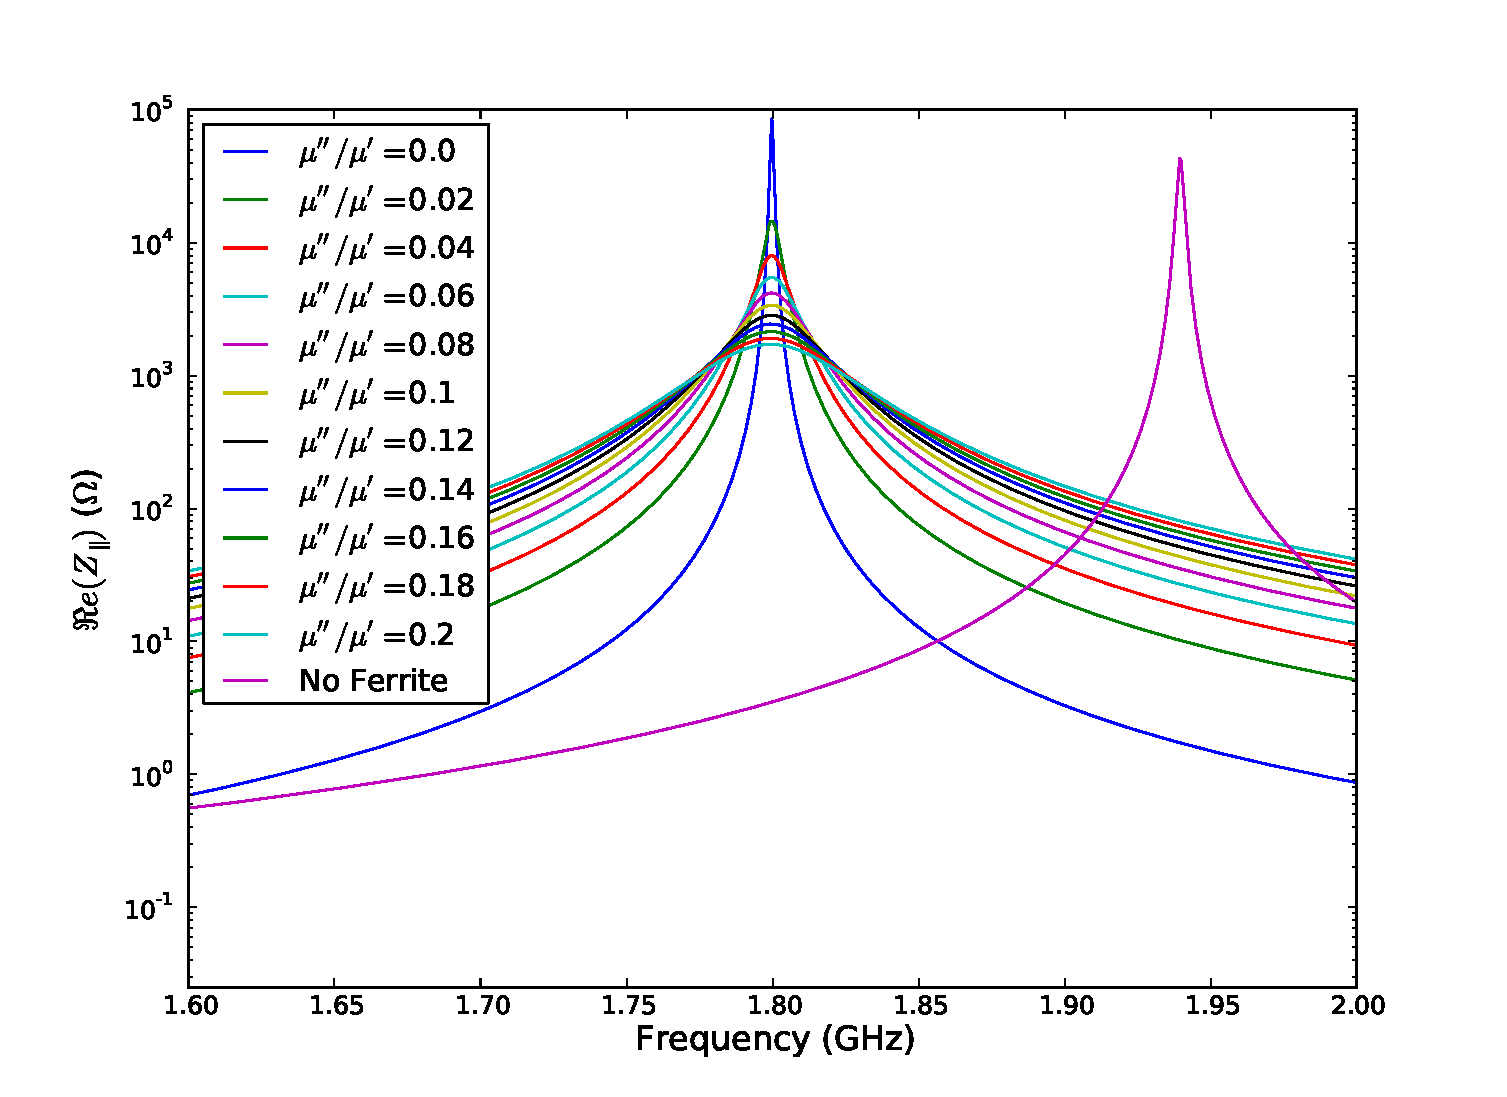
\includegraphics[width=0.7\textwidth]{Beam_Coupling_Impedance_Reduction_Techniques/figures/no_screen_long_imp_all.pdf}
\end{center}
\label{fig:no_screen_long_imp}
\caption{The real component of the longitudinal beam coupling impedance of a cavity without and with a damping material with $\epsilon^{'}=10$, $\mu^{'}=10$ and $\mu^{'}/\mu^{'}$ is varied. The non-damped cavity is shown for comparison. The change in resonance frequency and shunt impedance impedance is due to the increased $\epsilon^{'}$ of the damping material.}
\end{figure}

\begin{figure}
\subfigure[]{
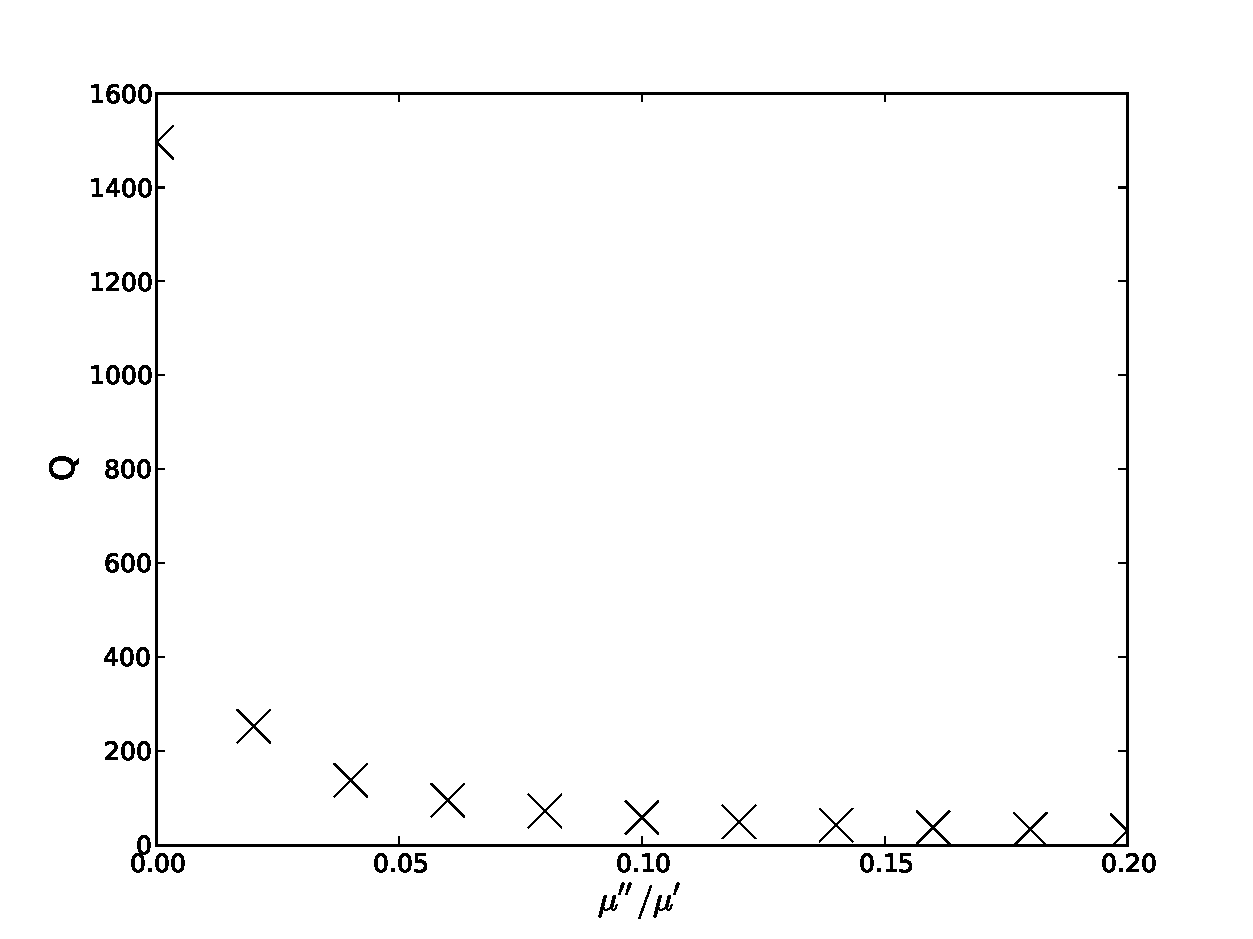
\includegraphics[width=0.45\textwidth]{Beam_Coupling_Impedance_Reduction_Techniques/figures/no_screen_loss_tan_vs_q.pdf}
\label{fig:cav_ferr_no_shield_tan_v_q}
}
\subfigure[]{
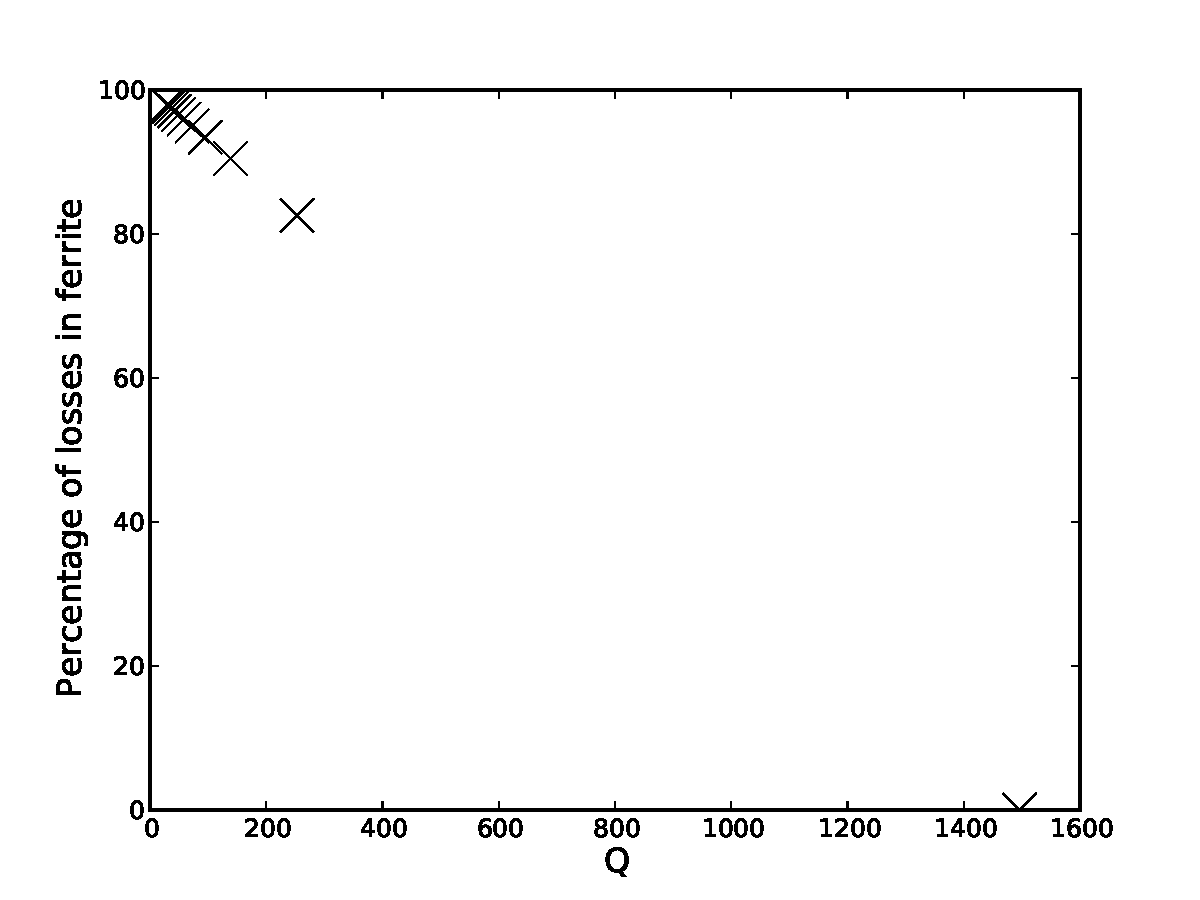
\includegraphics[width=0.45\textwidth]{Beam_Coupling_Impedance_Reduction_Techniques/figures/no_screen_q_vs_loss_ferr.pdf}
\label{fig:cav_ferr_no_shield_q_v_loss_ferr}
}
\label{fig:no_screen_res_alterations}
\caption{\ref{fig:cav_ferr_no_shield_tan_v_q} The reduction in the Q of the cavity resonance with the increasing loss tangent of the ferrite damping, showing a strong decrease of the resonant Q with a small increase in loss tangent. \ref{fig:cav_ferr_no_shield_q_v_loss_ferr} The percentage of the power loss in the ferrite as the resonant Q decreases. this can be seen to tend towards 100\% as the Q approaches 0.}
\end{figure}

\begin{figure}
\begin{center}
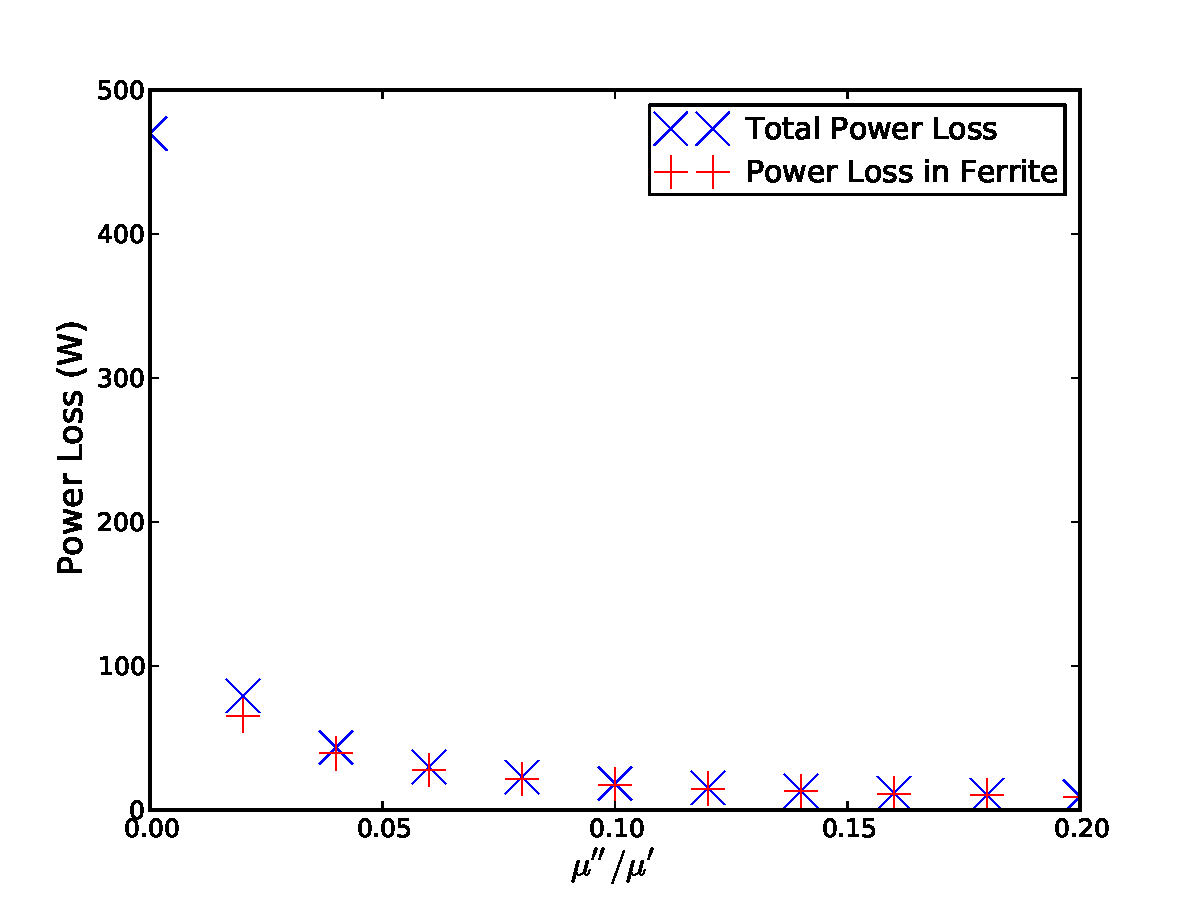
\includegraphics[width=0.7\textwidth]{Beam_Coupling_Impedance_Reduction_Techniques/figures/no_screen_loss_tan_vs_power.pdf}
\end{center}
\label{fig:no_screen_loss_tan_v_power}
\caption{The power loss due to  a beam with $1.15 \times 10^{11}$ particles per bunch, 288 bunches, a ring circumference 6911m and a bunch length $4\sigma = 0.04m$ assuming a gaussian bunch distribution in the unscreened cavity.}
\end{figure}

For the case of the shielded ferrite, the real component of the beam coupling impedance is shown in Fig.~\ref{fig:screen_long_imp}. As with the case of the unshielded ferrite, the addition of the damping material causes a decrease in the resonant frequency of the cavity mode, again due to the addition of a material with $\epsilon_{r} > 1$. In addition, the shielding causes a further decrease in the resonant frequency, in this case due to the rearrangement of the field lines due to the changed boundary conditions.

As can be seen from Fig.~\ref{fig:cav_ferr_shield_tan_v_q} the decrease in the Q of the resonance by the increasing more lossy ferrite follows a similar pattern to that shown by the unshielded structure, as is the increase in the percentage of power loss in the ferrite for the increasing damping of the resonance, shown in Fig.~\ref{fig:cav_ferr_shield_q_v_loss_ferr}. The corresponding change in the power loss in both the cavity as a whole and the ferrite is shown in Fig.~\ref{fig:screen_loss_tan_v_power}. As with the unscreened case, the power lost in the ferrite rapidly converges with the power loss in the entire cavity, indicating that magnetic losses are dominating the losses.	

\begin{figure}
\begin{center}
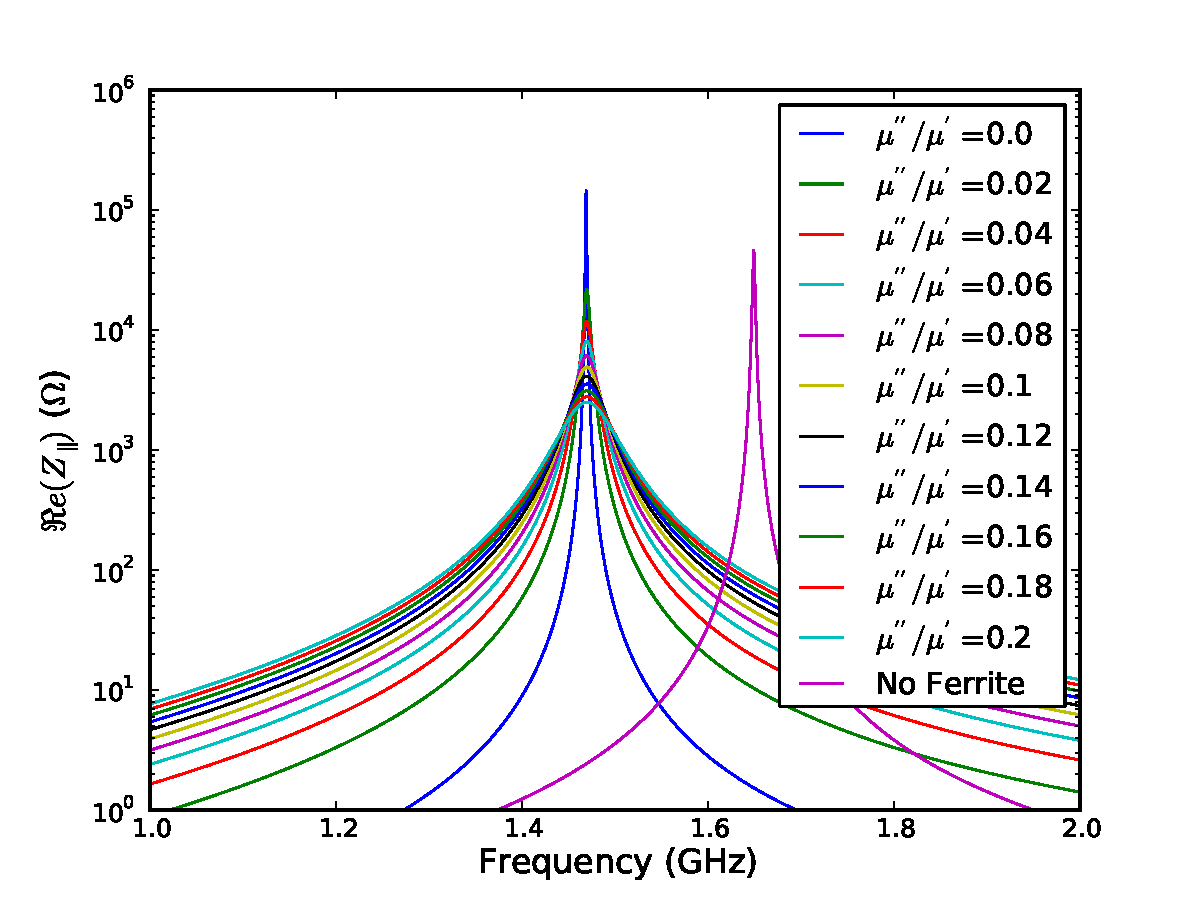
\includegraphics[width=0.7\textwidth]{Beam_Coupling_Impedance_Reduction_Techniques/figures/screen_long_imp_all.pdf}
\end{center}
\label{fig:screen_long_imp}
\caption{The real component of the longitudinal beam coupling impedance of a cavity without and with shielded damping material with $\epsilon^{'}=10$, $\mu^{'}=10$ and $\mu^{'}/\mu^{'}$ is varied. The non-damped cavity is shown for comparison. The change in resonance frequency and shunt impedance impedance is due to the increased $\epsilon^{'}$ of the damping material.}
\end{figure}


\begin{figure}
\subfigure[]{
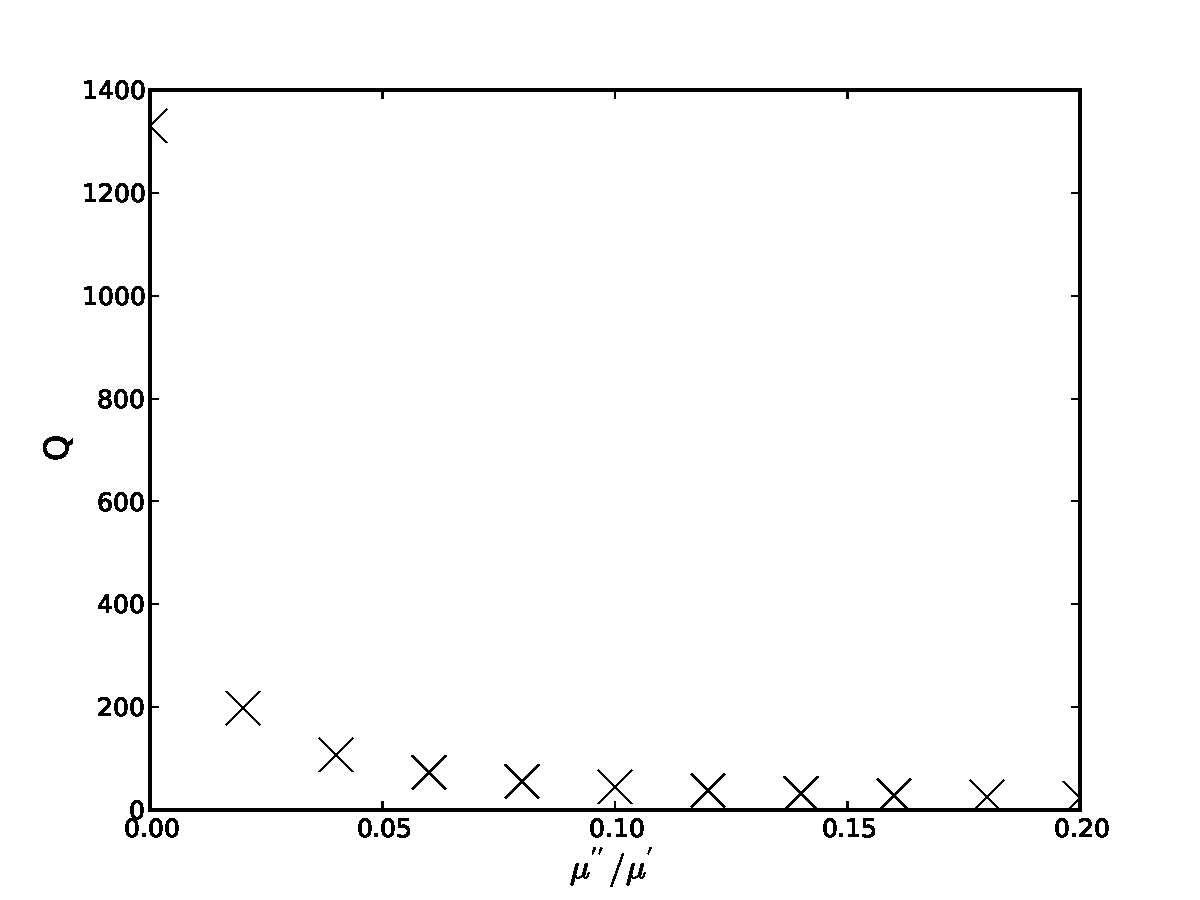
\includegraphics[width=0.45\textwidth]{Beam_Coupling_Impedance_Reduction_Techniques/figures/screen_loss_tan_vs_q.pdf}
\label{fig:cav_ferr_shield_tan_v_q}
}
\subfigure[]{
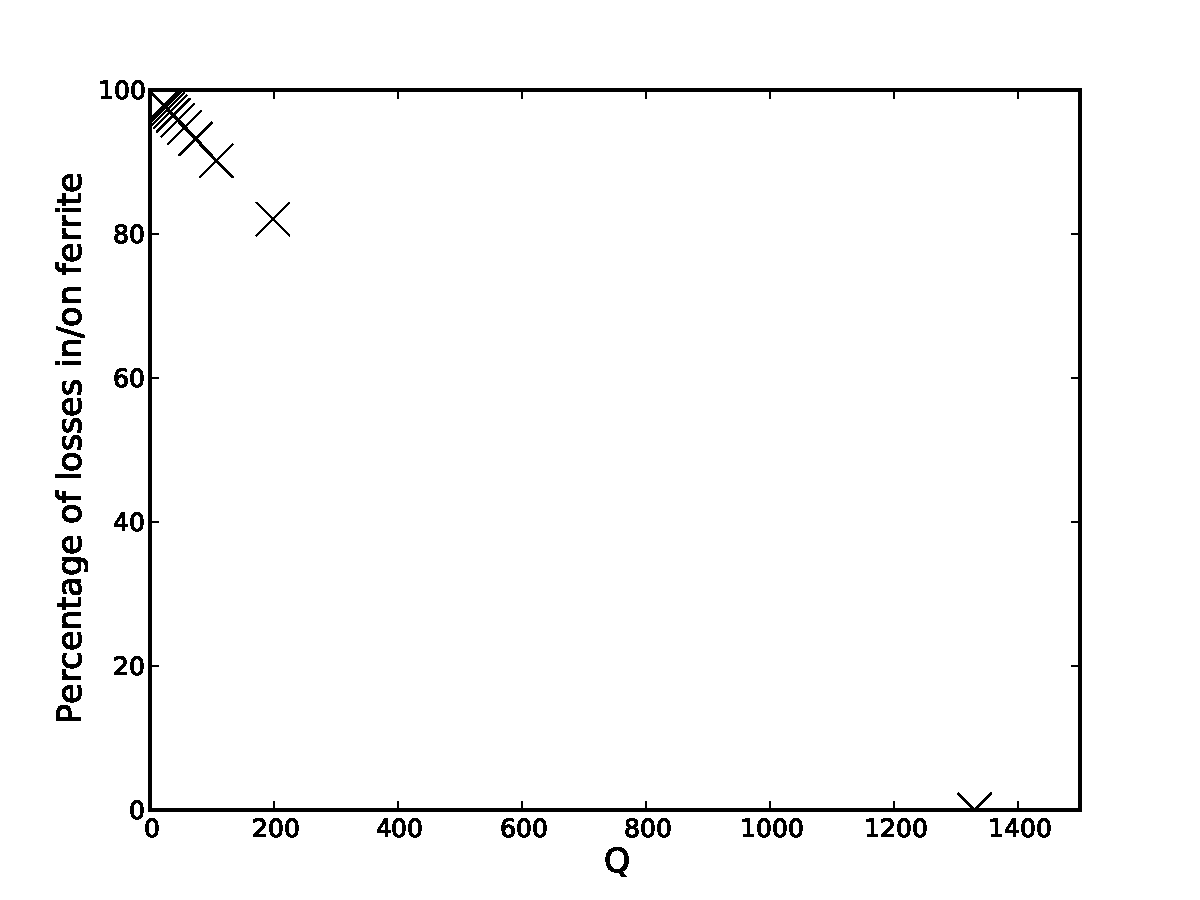
\includegraphics[width=0.45\textwidth]{Beam_Coupling_Impedance_Reduction_Techniques/figures/screen_q_vs_loss_ferr.pdf}
\label{fig:cav_ferr_shield_q_v_loss_ferr}
}
\label{fig:screen_res_alterations}
\caption{\ref{fig:cav_ferr_shield_tan_v_q} The reduction in the Q of the cavity resonance with the increasing loss tangent of the ferrite damping, showing a strong decrease of the resonant Q with a small increase in loss tangent. \ref{fig:cav_ferr_shield_q_v_loss_ferr} The percentage of the power loss in the ferrite as the resonant Q decreases. this can be seen to tend towards 100\% as the Q approaches 0.}
\end{figure}

\begin{figure}
\begin{center}
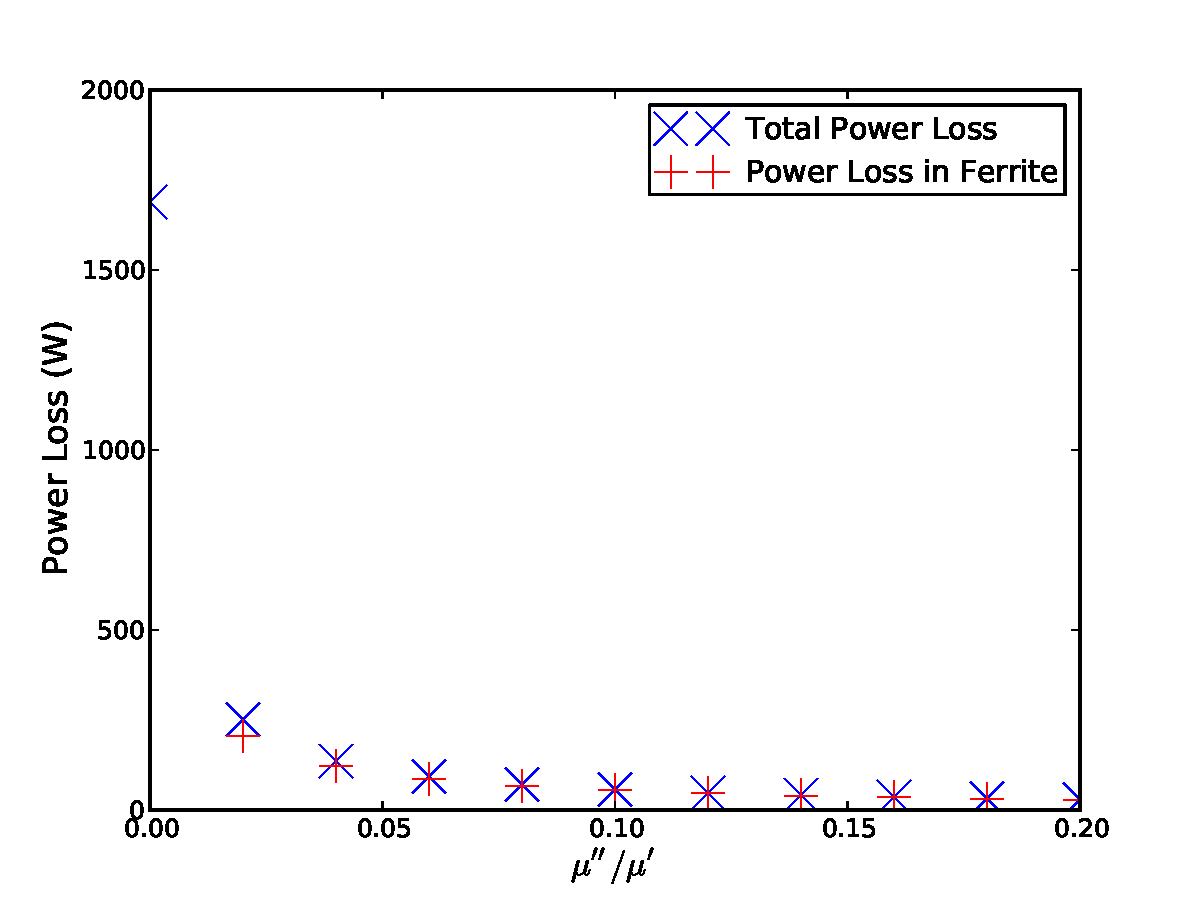
\includegraphics[width=0.7\textwidth]{Beam_Coupling_Impedance_Reduction_Techniques/figures/screen_loss_tan_vs_power.pdf}
\end{center}
\label{fig:screen_loss_tan_v_power}
\caption{The power loss due to a beam with $1.15 \times 10^{11}$ particles per bunch, 288 bunches, a ring circumference 6911m and a bunch length $4\sigma = 0.04m$ assuming a gaussian bunch distribution in the screened cavity.}
\end{figure}

From these results it can thus be seen that the inclusion of the shielding does not substantially effect the losses due to strong cavity resonances, whilst aiding in reducing the effects of image current flowing through the ferrite (a broadband effect, and thus not considered in the eigenmode simulations). In addition, we see that if the cavity mode is strongly damped by the presence of ferrite (i.e. the $Q$ is reduced by a factor 20 or so) it should be expected that the vast majority of the remaining power lost by particles interacting with the cavity resoance should ultimately be lost in the damping material. 